\documentclass[a4paper, 12pt]{article}
\usepackage[T1]{fontenc}
\usepackage{lmodern}
\usepackage{color}
\usepackage{amsfonts}
\usepackage{epstopdf}
\usepackage{matlab}
%\documentclass{book}
\usepackage{blindtext}
\usepackage{hyperref}
\usepackage[brazil]{babel}
\usepackage{amssymb}
\usepackage[utf8]{inputenc}
\usepackage{amsmath}
\usepackage{indentfirst}
\usepackage{graphicx}
\usepackage{multicol,lipsum}
\usepackage[a4paper,
top=3cm, left=3cm, bottom=3cm, right=3cm]{geometry}
\usepackage{setspace}
\usepackage{multirow}
\usepackage{float}
\usepackage[dvipsnames]{xcolor}
\usepackage[table]{xcolor}
%\usepackage{pdflscape}
\usepackage[DIV=15]{typearea}
\usepackage[nottoc]{tocbibind}
\usepackage[sort,numbers]{natbib}
%\usepackage{cite}
\usepackage{matlab}

\usepackage[utf8]{inputenc}
\usepackage[T1]{fontenc}
\usepackage{lmodern}
\usepackage{graphicx}
\usepackage{color}
\usepackage{hyperref}
\usepackage{amsmath}
\usepackage{amsfonts}
\usepackage{epstopdf}
\usepackage[table]{xcolor}
\usepackage{matlab}


\documentclass[letterpaper]{article}
% bib pack %%%%%%%%%%%%%%%%%%%%%%%%%%%%%%%%%%%%%%%%%%%%%%%%%%%%%%%%%%%%%%%%%%%%%
\usepackage[utf8]{inputenc}
\usepackage{geometry}
    \geometry{left=3cm,right=2cm,top=2cm,bottom=2cm}
%
\usepackage[spanish]{babel}
%
\usepackage[fixlanguage]{babelbib}
    \bibliographystyle{babunsrt}
%
\usepackage{url}

\begin{document}
%\maketitle

\begin{titlepage}
	\begin{center}
		

\vspace{10pt}
%\begin{figure}[H][!ht]
%\centering
%
\includegraphics{puc-rio-logo.png}

%\end{figure}
\begin{figure}[!ht]
\centering

\includegraphics{images/puc-rio-logo.png}
\end{figure}
\huge{Dinâmica de Sistemas}
        \vspace{70pt}
        
		\textbf{ENG1730}
		\textbf{\large{\\ }}
		
		\vspace{30pt}
		\textbf{\small{\\Lista 05}}
		\vspace{75pt}
		
	\end{center}
	
	\begin{flushleft}
		\begin{tabbing}
			Aluno(a)\qquad\qquad\=\>Paloma Fernanda Loureiro Sette - 1621595\\
			
			Professor(a)\>João Carlos Virgolino Soares\\
	\end{tabbing}
		  
	\end{flushleft}
	\begin{center}
		%\vspace{\fill}
		\vspace{215pt}
		Rio de Janeiro, 04 de Outubro de 2022
	\end{center}
\end{titlepage}
%%%%%%%%%%%%%%%%%%%%%%%%%%%%%%%%%%%%%%%%%%%%%%%%%%%%%%%%%%%
\newpage
\tableofcontents
\thispagestyle{empty}

\newpage
\pagenumbering{arabic}

\newpage

%\newcommand{\listequationsname}{Lista de Equações}
%\newlistof{myequations}{equ}{\listequationsname}
%\newcommand{\myequations}[1]{%
%\addcontentsline{equ}{myequations}{\protect\numberline{\theequation}#1}\par}

%\listofmyequations
\newpage


\newpage

\listoffigures
\thispagestyle{empty}

\newpage
%%%%%%%%%%%%%%%%%%%%%%%%%%%%%%%%%%%%%%%%%%%%%%%%%%%%%%%%%
%%%%%%%%%%%%%%%%%%%%%%%%%%%%%%%%%%%%%%%%%%%%%%%%%%%

\newpage

\thispagestyle{empty}

\newpage

\section{Introdução}
Este relatório refere-se ao quinto trabalho da disciplina de Dinâmica de Sistemas, ENG1730, de 2022.2. Trataremos da modelagem de um sistema composto por um carro contendo um pêndulo simples, mola e amortecedor.

\section{Questão 01}
A figura a seguir mostra uma haste de massa m acoplada a uma base móvel de massa $M$. A base está atrelada a uma mola de constante $k_T$ e a um amortecedor de constante $b_T$. O eixo de rotação entre o pêndulo e a base possui atrito viscoso de coeficiente $b_R$ e uma rigidez rotacional $k_{R}$.

\begin{figure}[H]
\centering

\includegraphics[scale = 0.7]{images/sistema.png}
\label{filtro1}
\caption{Carro contendo o pêndulo simples, mola e amortecedor}
\end{figure}

As dimensões da haste são:

\begin{figure}[H]
\centering
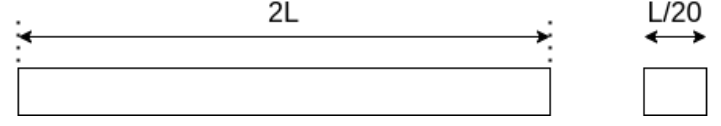
\includegraphics[scale = 0.7]{images/dim_haste.png}
\label{filtro1}
\caption{Dimensões da haste}
\end{figure}

Devemos resolver os itens propostos, organizados em tópicos a seguir.


\subsection{Modelo matemático do sistema}
\subsection{Resposta Dinâmica do Sistema - Simulink}

A partir do modelo matemático, encontrar a resposta dinâmica do sistema (posição e velocidade do carro, ângulo e velocidade angular da haste) usando o \textbf{Simulink}, com os seguintes parâmetros iniciais:\\


$\theta_0 = 10 \>\ graus$\\
$k_T = 0 \>\ N/m$\\
$b_T = 0.45\>\ N/(m/s)$\\
$k_R = 0 \>\ Nm/rad$\\
$b_R = 10.3 \>\ Nm/(rad/s)$\\
$M = 2 \>\ kg$\\
$m = 1.5 \>\ kg$\\
$F = 0\>\ N$\\
$L = 3 \>\ m$\\
$t = 20 \>\ s$\\




\subsection{Resposta Dinâmica do Sistema - Simscape Multibody}

Encontre a resposta dinâmica do sistema usando o Simscape Multibody, com os mesmos parâmetros do item anterior.

\subsection{Definição dos Parâmetros}

Criamos um script no MATLAB para definir os parâmetros do sistema e rodar os dois modelos
(Simulink e Simscape).

\subsection{Respostas Gráficas}

No script criado, geramos os gráficos de posição/velocidade do carro e ângulo da haste em função do tempo. Enviamos a resposta do Simulink para o workspace do MATLAB e plotamos no script.

\subsection{Análise do Funcionamento do Sistema}
%Explique o comportamento do sistema. Compare os resultados obtidos no Simulink e no Simscape Multibody;

\subsection{Redefinição dos Parâmetros - Repouso da Haste < 5 s}
Redefinimos os parâmetros para que a haste fique em repouso em menos de 5 segundos. %Explique a escolha de parâmetros e plote os resultados no script.

\subsection{Redefinição dos Parâmetros - Repouso da Haste < 10 s}
Redefinimos os parâmetros para que a haste fique em repouso em menos de 10 segundos. %Explique a escolha de parâmetros e plote os resultados no script.

\subsection{Redefinição dos Parâmetros - Comportamento Estável}
Fizemos a redefinição dos parâmetros para que o sistema se comporte como um pêndulo simples de base estática. Testamos com $\theta_0 = 30 \>\ graus$. %Explique a escolha de parâmetros e plote os resultados no script.


\subsection{Redefinição dos Parâmetros - Sistema massa-mola-amortecedor}
Redefinimos os parâmetros para que o sistema se comporte como um sistema massa-mola-amortecedor puramente oscilatório. Testamos com uma força $F$ não-nula. %Explique a escolha de parâmetros e plote os resultados no script.


\newpage
% REFERENCIAS %%%%%%%%%%%%%%%%%%%%%%%%%%%%%%%%%%%%%%%%%%%%%%%%%%%%%%%%%%%%%%
    \nocite{*}
    \bibliography{src/bibliography}
    
\end{document}
\section{Referências Bibliográficas}



\end{document}